\documentclass[10pt,a4paper]{article}

\usepackage[utf8]{inputenc}
\usepackage[T1]{fontenc}
\usepackage[english]{babel}
\usepackage[left=3.5cm,top=2cm,right=3.5cm,bottom=2cm]{geometry}

\usepackage{amsmath}
\usepackage{amsfonts}
\usepackage{amssymb}
\usepackage{amsopn}
\usepackage{amsthm}
\usepackage[hidelinks]{hyperref}
\usepackage{cleveref}
\usepackage{fancyvrb}
\usepackage{tikz}
\usepackage[justification=centering]{caption}
% \patchcmd{\thebibliography}{\chapter*}{\section*}{}{}
\usepackage[super]{nth}
\usepackage{textcomp}
\usepackage{enumitem}
\usepackage{doi}
\usepackage{mathrsfs}
\usepackage{siunitx}
\setlist{nosep}
% \usepackage[justification=justified,singlelinecheck=false]{caption}
\usepackage{subcaption}


\theoremstyle{plain}
\newtheorem{thm}{Theorem}[section]
\newtheorem{prop}[thm]{Property}
\newtheorem{lem}[thm]{Lemma}
\newtheorem{cor}{Corollary}[thm]

\theoremstyle{definition}
\newtheorem{defn}{Definition}[section]
% \newtheorem{axi}{Axiom}[chapter]
\newtheorem{eqn}[thm]{Equation}

\theoremstyle{remark}
\newtheorem*{rem}{Remark}


\setcounter{secnumdepth}{3}
\setcounter{tocdepth}{1}
% \renewcommand\thesection{\arabic{section}}

\newcommand{\R}{\ensuremath{\mathbb{R}}}
\newcommand{\Rb}{\ensuremath{\overline{\mathbb{R}}}}
\newcommand{\N}{\ensuremath{\mathbb{N}}}
\newcommand{\Q}{\ensuremath{\mathbb{Q}}}
\newcommand{\Z}{\ensuremath{\mathbb{Z}}}
\newcommand{\C}{\ensuremath{\mathbb{C}}}
\newcommand{\U}{\ensuremath{\mathbb{U}}}
\newcommand{\F}{\ensuremath{\mathbb{F}}}
\newcommand{\K}{\ensuremath{\mathbb{K}}}
\newcommand{\TODO}{\textbf{TODO}}


\newcommand\eqdef{\stackrel{\mathclap{\mbox{\tiny def}}}{=}}


\sisetup{inter-unit-product=\ensuremath{{}\cdot{}}}

\newcommand{\ket}[1]{|#1\rangle}
\newcommand{\bra}[1]{\langle#1|}
\newcommand{\braket}[2]{\langle#1|#2\rangle}

\newcommand{\dd}{\mathrm{d}}
\newcommand{\der}[2]{\frac{\dd{#1}}{\dd{#2}}}
\newcommand{\dern}[3]{\frac{\dd^{#3} #1}{\dd{#2}^{#3}}}
\newcommand{\dpar}[2]{\frac{\partial{#1}}{\partial{#2}}}
\newcommand{\dparn}[3]{\frac{\partial^{#3} {#1}}{\partial{#2}^{#3}}}

\renewcommand{\geq}{\geqslant}
\renewcommand{\leq}{\leqslant}

\newcommand{\mat}[1]{\begin{pmatrix}#1\end{pmatrix}}
\newcommand{\bs}{\boldsymbol}

\DeclareMathOperator{\cov}{cov}
\DeclareMathOperator{\Tr}{Tr}
\DeclareMathOperator{\argmax}{arg\,max}
\DeclareMathOperator{\argmin}{arg\,min}
\DeclareMathOperator{\rk}{rk}
\DeclareMathOperator{\Span}{Span}
\DeclareMathOperator{\dom}{dom}


\newcommand{\class}[1]{{\mathscr{C}^{#1}}}

\newcommand{\trnorm}[1]{\frac{#1}{\Tr\left({#1}\right)}}
\newcommand{\pr}{_{||}}
\newcommand{\inv}{^{-1}}
\newcommand{\ml}{_{M\!L}}


\newcommand{\maxim}[3]{\begin{cases}
    \mathbf{maximize}\,\quad #1& \mathbf{on}\; #2\\
    \mathbf{subject\;to}\quad #3
  \end{cases}}
\newcommand{\maximf}[2]{\begin{cases}
    \mathbf{maximize}\,\quad #1& \mathbf{on}\; #2
  \end{cases}}
\newcommand{\maxima}[3]{\begin{cases}
    \mathbf{maximize}\,\quad #1& \mathbf{on}\; #2\\
    \mathbf{subject\;to}\quad \begin{aligned}[t]#3\end{aligned}
  \end{cases}}

\newcommand{\minim}[3]{\begin{cases}
    \mathbf{minimize}\;\,\quad #1& \mathbf{on}\; #2\\
    \mathbf{subject\;to}\quad #3
  \end{cases}}
\newcommand{\minimf}[2]{\begin{cases}
    \mathbf{minimize}\,\quad #1& \mathbf{on}\; #2
  \end{cases}}
\newcommand{\minima}[3]{\begin{cases}
    \mathbf{minimize}\;\,\quad #1& \mathbf{on}\; #2\\
    \mathbf{subject\;to}\quad \begin{aligned}[t]#3\end{aligned}
  \end{cases}}

\newcommand{\gap}{\hspace{0.5cm}}
\newcommand{\twoline}{\vphantom{\frac\int\int}}

\graphicspath{{../img/}}

\title{Error estimation in maximum-likelihood reconstruction for quantum state tomography}
\author{Thibaut Pérami, Igor Dotsenko, Pierre Rouchon}

\makeatletter
\hypersetup{
  pdftitle = {\@title},
  pdfauthor = {\@author},
  pdfsubject = {Quantum state tomography}
}
\makeatother

\begin{document}

\maketitle

\newcommand{\fset}{\ensuremath{\mathop{\text{\textquotesingle}}}}




\section*{Abstract}

The maximum likelihood estimator is often used in to reconstruct state in the
context of quantum state tomography. The formulas used by physicist are based on
asymptotic development of multi-dimensional Laplace integrals. The results
obtained in previous work allow to provably retrieve the value and first-order
error estimation of the evaluation of any quantum observable on the
reconstructed quantum state. Those results hold even when on the boundaries of
the integration domain. However in the context of Quantum Thermodynamics,
physicists need to evaluate non linear function of the quantum observable. In
particular Von-Neumann entropy whose first order derivative goes to infinity on
the edge of the domains. In this paper we prove again expansion of those
integral with minimal hypothesis. We also prove variation of such expansion that
are applicable to the Von-Neuman Entropy. In addition we have some informal proposition
about how to handle the case where the information obtained on the quantum state
is incomplete.


\section{Introduction}

\TODO

\subsection{Previous Work}

Previous results.

\subsection{Goal}

\section{Generic Laplace expansion of integrals}

In this section we generalize the problem to generic expansion in $\R^n$. Doing
it in $\R^n$ is sufficient for it to be usable in any differential variety like
$\mathcal{D}$. Thanks to a trick we'll see in \cref{sec:app} (from \cite{SPRAL17}), we only need to
care about boundaries of dimension one less that the main dimension. The
generalized integral we study is:

\[\int_{z \in U} g(z)e^{N\!f(z)} \dd z\]

where $f$ is concave and when $N$ goes to infinity. Intuitively, the result
expansion will use only value around the maximum of $f$
We do not prove all the possible case of this expansion, but only the ones that
are useful in the quantum setting.

\subsection{In the interior}

We start by abstracting $f$ even mode with $f(z) = - \frac {\|z\|^2}2$ and start
the asymptotic expansion. $U$ always represent an open set of $\R^n$.

\begin{thm}\label{thm:asy1}
  Let $g : U \to \R$ be a function of class $\class 1$ on $U$ a neighborhood of 0. If $g(0)
  \neq 0$, we have, as $N \to \infty$:
  \[\int_{z \in U} g(z)e^{-\frac N2\|z\|^2} \dd z = g(0){\left(\frac
        {2\pi}{N}\right)}^{\frac n 2} +
    O\left({N^{-\frac n 2 -1}}\right)\]
\end{thm}

\begin{proof}
  We can decompose $g$ in $g(z) = g(0) + h(z)$ with $h(z) = O(\|z\|)$ as $g$ is
  $\class{1}$ in 0, thus:
  \[\int_{z \in U} g(z)e^{-\frac N2\|z\|^2} \dd z = g(0)\int_{z \in U} e^{-\frac
      N2\|z\|^2} \dd z + \int_{z \in U} h(z)e^{-\frac N2\|z\|^2} \dd z.\]
  Furthermore,
  \begin{align*}
    \left |\int_{z \in U} h(z)e^{-\frac N2\|z\|^2} \dd z\right|
    &\leq C \int_{z \in U} \|z\|e^{-\frac N2\|z\|^2} \dd z\\
    &\leq C \int_{z \in \R^n} \|z\|e^{-\frac N2\|z\|^2} \dd z\\
    &\leq CA_n \int_{r \in \R_+} r^{n+1}e^{-\frac N2 r^2} \dd r\\
    &\leq CA_n \int_{r \in \R_+} r^{n+1}e^{-\frac N2 r^2} \dd r\\
    &\leq CA_n \int_{r \in \R_+} r^{n+1}e^{-\frac N2 r^2} \dd r\\
    &\leq CA_n \left ( \frac2N\right)^{\frac n2+1}\int_{s \in \R_+} s^{n+1}e^{-s^2} \dd s
    & {\textstyle\left (s = \sqrt{\frac N2} r\right)} \\
    &\leq O\left({N^{-\frac n 2 -1}}\right)
  \end{align*}

  where $C$ is the constant such that $|h(z)| \leq C \|z\|$, $A_n$ is the surface
  of the hypersphere of $\R^n$.

  Additionally, up to exponentially small terms ($O(e^{N\delta})$ for a given $\delta$), we have:
  \[g(0)\int_{z \in U} e^{-\frac
      N2\|z\|^2} \dd z \approx g(0)\int_{z \in \R^n} e^{-\frac
      N2\|z\|^2} \dd z = g(0) {\left(\frac
        {2\pi}{N}\right)}^{\frac n 2}\]

  By adding both equations, we get the theorem.
\end{proof}

\


However when $g(0) = 0$, the previous theorem does not give anymore the first
order term but just a bound on the integral which may not be very useful in
certain cases. We'll thus look in more details at the case $g(0) = 0$. We'll
assume additionally that $\nabla g = 0$, because that is what happens for our
cases that require that theorem.


\begin{thm}\label{thm:asy2}
  Let $g : U \to \R$ be a function of class $\class 3$ on $U$ a neighborhood of 0. If $g(0) = 0$
  and $\nabla g(0) = 0$, we have, as $N \to \infty$:
  \[\int_{z \in U} g(z)e^{-\frac N2\|z\|^2} \dd z = \frac{\Tr(\nabla^2 g(0))}{2N} {\left(\frac
        {2\pi}{N}\right)}^{\frac n 2} +
    O\left({N^{-\frac n 2 -2}}\right).\]
\end{thm}

\begin{proof}
  $g$ can be written $g(z) = \frac12\bra z \nabla^2 g(0) \ket z + O(\|z\|^3)$ because it
  is $\class 3$. The integral on the $O(\|z\|^3)$ part gives $O\left({N^{-\frac
        n 2 -2}}\right)$ with exactly the same method as in
  the precedent proof (replace $\|z\|$ by $\|z\|^3$ and $r^{n+1}$ by $r^{n+3}$.

  We can then use prove a little lemma to get the result:

  \begin{lem}\label{lem:gausssymtr}
    Let $S$ be an real symmetric matrix of dimension $n$, we have:
    \[\int_{z \in \R^n} \bra z S \ket z e^{-\frac N 2 \|z\|^2} \dd z =
      \frac{\Tr(S)}N {\left(\frac
          {2\pi}{N}\right)}^{\frac n 2} \]
  \end{lem}
  \begin{proof}[Lemma proof] If we take the spectral decomposition of $S$ and split the
    coordinate along $S$ eigenvectors, the result comes after some calculus.
  \end{proof}

  The application of the lemma with $S = \nabla^2 g(0)$ and the previous
  asymptotic bound added give the theorem.
\end{proof}

\

It is now time to replace the $-\|z\|^2$ by a generic concave function and to do
the actual change of variables.

\begin{thm}\label{thm:asymid}
  Let $U$ be an open set containing $0$. Let $f : U \to \R$ be a $\class 4$ function.
  Let $g : U \to \R$ be a $\class 1$ function.
  Assume that $f$ has a unique global non critical maximum in $0$
  ($\nabla f = 0$ and $\nabla^2 f < 0$). We have at $N \to \infty$:
  \[\int_{z \in U} g(z)e^{Nf(z)} \dd z = g(0)
    {\left(\frac {2\pi}{N}\right)}^{\frac n 2}
    \frac {e^{Nf(0)}}{\sqrt{\left|\det \nabla^2 f(0)\right|}}
    + O(e^{Nf(0)} N^{-\frac n 2 -1})\]

  Additionally, If $g(0) = 0$ and $\nabla g(0) = 0$, and $f \in \class 6$ and $g
  \in \class 3$, we have:

  \[\int_{z \in U} g(z)e^{N f(z)} \dd z =
    \frac{\Tr\left(-\nabla^2 g(0) {\left(\nabla^2 f(0)\right)}^{-1}\right)}{2N}
    {\left(\frac {2\pi}{N}\right)}^{\frac n 2}
    \frac {e^{Nf(0)}}{\sqrt{\left|\det \nabla^2 f(0)\right|}}
    + O\left(e^{Nf(0)}{N^{-\frac n 2 -2}}\right)\]
\end{thm}

\begin{proof}
  First we assume $f(0) = 0$ without loss of generality (it suffice to divide
  everything by $e^{Nf(0)}$). The Morse lemma (\ref{lem:morse}) tells us that
  there is a  neighborhood $V$ of 0 and
  a diffeomorphism $\psi : V \to V'$ with $\psi(0) = 0$ such that
  \[f(z) = - \frac12 \|\psi(z)\|^2 \gap \text{and}\gap \nabla \psi(0) =
    \sqrt{-\nabla^2 f}.\]

  Because the hessian of $f$ is negative definite in 0 and the maximum is unique,
  all values of $f$ outside of $V$ are below a
  constant $-\delta$. So all the part of the integral outside of $V$ are
  $O(e^{-N\delta})$ and thus negligible. We can now study the integral only on
  $V$. We can then make a change of variable on $\psi$:

  \[\int_{z \in V} g(z)e^{Nf(z)} = \int_{z \in V'}
    g(\psi^{-1}(z))e^{-\frac N2\|z\|^2} J(z) \dd z\]

  with $J(z) = |\det{\nabla \psi^{-1}}|$. We can then set $g_0(z) =
  g(\psi^{-1}(z))J(z)$, and look at the two cases:
  \begin{itemize}
  \item As $f \in \class 4$, we have $\psi \in \class 2$ (and thus also
    $\psi^{-1}$) and finally $J \in \class 1$, but $g$ is also in $\class 1$, so
    $g_0$ is in $\class 1$. We can then apply \cref{thm:asy1} and get the result
    we want with:
    \[g_0(0) = g(\psi^{-1}(0))J(0) = g(0)\frac 1 {\det {\nabla \psi(0)}} =
      \frac {g(0)}{\sqrt{\left|\det \nabla^2 f\right|}}
    \]


  \item As $f \in \class 6$, we have $\psi \in \class 4$ (and thus also
    $\psi^{-1}$) and finally $J \in \class 3$, but $g$ is also in $\class 3$, so
    $g_0$ is in $\class 3$. We can then apply \cref{thm:asy2} and get the result
    we want with:
    \[\nabla g_0^t = \nabla g^t \nabla \psi\inv \times J + g \circ \psi\inv
      \times \nabla J\]
    but as $g(0) = 0$, we have $g(\psi^{-1}(0)) = 0$ and furthermore $\nabla
    g(0) = 0$ so $\nabla (g \circ \psi^{-1})(0) = 0$. Finally, the only remaining term is:
    \begin{align*}
      \nabla^2 g_0(0))
      &= \nabla^2 (g \circ \psi\inv) \times J(0)\\
      &= {(\nabla \psi^{-1}(0))}^t\nabla^2 g(0) {(\nabla \psi^{-1}(0))} \times
        \frac {1}{\sqrt{\left|\det \nabla^2 f\right|}}
    \end{align*}
    If we put that to the trace, we get the result we wanted.
  \end{itemize}
\end{proof}


\subsection{On the boundaries}

As said earlier we can content ourselves with working on an hyperplane boundary.
So we'll take $U$ as subset of $\R_+ \times \R^n$ and work from there.

\begin{rem}
  All theorems work with $n = 0$ i.e on $\R_+$ alone. It suffice to note that the
  Lebesgue measure of the point in dimension 0 is 1 and all the proofs will work directly.
\end{rem}

\begin{thm}\label{thm:asyp1}
  Let U be an open bounded set of $\R_+ \times \R^n$ where $(0,0) \in U$. The $\R_+$
  coordinate will be $x$ and the $\R^n$ coordinate will be $z$. Let $g : U \to
  \R$ be a $\class 1$ function. The derivatives against the edge i.e on $x$ when
  $x=0$ are
  taken as one-sided derivatives. We have as $N \to \infty$:

  \[\int_{(x,z) \in U} x^m g(x,z)e^{-N(x + \frac 12 \|z\|^2)} \,\dd x\, \dd z =
    g(0,0)\,m! {(2\pi)}^{\frac n 2} N^{-\frac n 2 - m - 1} + O(N^{-\frac n 2 - m - 2})\]
\end{thm}

\begin{proof} We can restrict ourselves to a
  rectangular set $U' = [0,\eta) \times U_z \subset U$ with the usual argument:
  the value inside
  the integral on $U \setminus U'$ is $O(e^{-N\delta}$ and $U$ is
  bounded so the integral on $U \setminus U'$ is exponentially negligible. We
  further restrict $U'$ such that $g$ and $g'$ are bounded on $U'$ (by taking the
  interior of a compact neighborhood included in $U$).

  Here we decompose $g$ in $g(x,z) = h(z) + x g_1(x,z)$ with $h(z) = g(0,z)$ (\cref{lem:dec}). As
  $g_1$ is bounded on $U'$, we have:
  \begin{align*}
    \int_{(x,z) \in U'} x^{m+1}g_1(x,z)e^{-N(x + \frac 12 \|z\|^2)} \,\dd x\, \dd z
    &\leq
      \|g_1\|_\infty\int_{(x,z) \in U'} x^{m+1}e^{-N(x + \frac 12 \|z\|^2)} \,\dd x\, \dd z\\
    &=O(N^{-\frac n 2 - m - 2})
  \end{align*}
  This is because we can split the integral on $x$ and $z$ and then do an
  appropriate change of variable to get $N$ out of both resulting integrals.
  On the other hand, thanks to \cref{thm:asy1} and the relation between the $\Gamma$
  function and the factorial, we have:
  \begin{align*}
    \int_{(x,z) \in U'} x^{m}h(z)e^{-N(x + \frac 12 \|z\|^2)} \,\dd x\, \dd z
    &= \int_0^\eta x^{m}e^{-Nx} \,\dd x \times
      \int_{z \in U_z} h(z)e^{-\frac N2 \|z\|^2} \, \dd z\\
    &= m! N^{-m-1} \times( h(0){\left(\frac
      {2\pi}{N}\right)}^{\frac n 2} +
      O\left({N^{-\frac n 2 -1}}\right))
  \end{align*}

  We get the theorem by adding both equations.
\end{proof}

\

\begin{thm}\label{thm:asyp2}
  If we add to the previous theorem the hypothesis that $g(0) = 0$, $\nabla g(0) =
  0$ and $g$ is $\class 2$ and in particular $\class 3$ on the
  variable $z$ (i.e.\ for any $x$, $z \mapsto g(x,z) \in \class 3$), we have:
  \[\int_{(x,z) \in U} x^m g(x,z)e^{-N(x + \frac 12 \|z\|^2)} \,\dd x\, \dd z
    = \frac{m!\Tr\left(\dparn g z 2\right)}{2N^{m+2}}
    {\left(\frac {2\pi}{N}\right)}^{\frac n 2}
    + O\left({N^{-\frac n 2 -m -3}}\right)\]

  Where $\dparn g z 2$ is the partial hessian on $z$.
\end{thm}

\begin{proof}
  We use the same $U'$ as in last proof (same shape and boundedness on $g$, $g'$
  and $g''$).
  By applying \cref{lem:dec} twice, we get
  \[g(x,z) = h(z) + x^2g_2(x,z)\]
  For that same reason as in previous proof, The integral on $x^2g_2$ is
  $O(N^{-\frac n2 - m - 3})$. We can then, like the previous proof, split the
  integral on $h(z)$ and use \cref{thm:asy2} to get the result.
\end{proof}

Like in the previous section we now need to take care about a generic function
$f$ in the exponential. We can't use the \cref{thm:asymid} because it assumes a
null gradient for $f$ but here $\dpar f x$ could be negative. In practice we
only care about the case where is indeed negative, otherwise we can adapt \cref{thm:asymid}.

\begin{thm}\label{thm:asypmid}
  Let U be an open set of $\R_+ \times \R^n$ where $(0,0) \in U$. The $\R_+$
  coordinate will be $x$ and the $\R^n$ coordinate will be $z$. Let $f:U \to \R$
  be a function of class $\class 4$ and $g : U \to
  \R$ be a function of class $\class 1$. The derivative against the edge i.e on $x$ are
  taken as one-sided derivative. Assume that $f$ has a global non-critical
  maximum in $0$ so that $\dpar f z(0) = 0$ and $\dparn f z 2(0) < 0$. Furthermore, we
  assume that $\dpar f x(0) < 0$. We have as $N \to \infty$:
  \begin{multline*}
    \int_{(x,z) \in U} x^m g(x,z)e^{Nf(x)} \,\dd x\, \dd z =\\
    \frac{g(0,0)\,m! {(2\pi)}^{\frac n 2}}{N^{\frac n 2 + m + 1}} \times
    \frac{e^{Nf(0,0)}}
    {\sqrt{\left|\det \dparn f z 2\right|} \left(-\dpar f x\right)^{m+1}}
    + O(e^{Nf(0,0)}N^{-\frac n 2 - m - 2})
  \end{multline*}

  Additionally, if $g(0) = 0$, $\nabla g(0) = 0$, $g$ is $\class 2$ and in
  particular $g$ is $\class 3$ on
  variable $z$ and $f$ is $\class 6$, We have as $N \to \infty$:
  \begin{multline*}
    \int_{(x,z) \in U}
     x^m g(x,z)e^{Nf(x)} \,\dd x\, \dd z =\\
     \frac{m!\Tr\left(\dparn g z 2 \left( \dparn f z 2 \right)\inv\right)}{2N^{m+2}}
    \times
    \frac{{\left(\frac {2\pi}{N}\right)}^{\frac n 2}e^{Nf(0,0)}}
    {\sqrt{\left|\det \dparn f z 2\right|} \left(-\dpar f x\right)^{m+1}}
    + O\left(e^{Nf(0,0)}{N^{-\frac n 2 -m -3}}\right)
  \end{multline*}
\end{thm}

\begin{proof}
  We start by supposing $f(0,0) = 0$ by dividing everything by $e^{Nf(0,0)}$.

  We now do a change a variable to bring back $f$ to be $-x -\frac12\|z\|^2$ like in
  the proof of \cref{thm:asymid}.
  To that change of variable we decompose $f$ in $f(x,z) = h(z) + xf_1(x,z)$
  with $h(z) = f(0,z)$. The change of variable $\tilde x = xf_1(x,z)$ and
  $\tilde z = \psi(z)$ where $\psi$ is the Morse lemma (\ref{lem:morse}) decomposition of $h$ will
  give the right result. Doing the actual variable change and computing the
  Jacobian is left to the reader.
  The regularity analysis is the same as in \cref{thm:asymid}

  \TODO{} Maybe we should actually do it.
\end{proof}




\section{Application to quantum state tomography}
\label{sec:app}

\TODO{} $\rho\ml$ and $\ell$ must be already introduced in the introduction

Here we can finally apply all those asymptotic theorems to our case. I first recall the
notations. For $h : \mathcal{D} \to \R$, we define
\begin{equation}
I_h(N) = \int_{\rho\in\mathcal{D}} h(\rho) e^{N\ell(\rho)} P_0(\rho) \dd \rho
\end{equation}
where $P_0$ is the prior probability distribution on density matrices.
So that we have its expectation
\begin{equation}
E_h(N) = \frac{I_h(N)}{I_1(N)}.
\end{equation}

Its variance is the expectation of:
\begin{equation}
h_V = {\left(h - \lim_{N \to \infty} E_h(N)\right)}^2
\end{equation}

We make some technical assumptions such as:
\begin{itemize}
\item $P_0(\rho\ml) > 0$: If our estimator has a null-probability, the prior
  distribution doesn't make much sense.
\item $P_0$ is of class $\class 3$: This is necessary for the various asymptotic
  developments. As $P_0$ is often the uniform distribution, this is not a strong requirement.
\item $\mathcal{D} = \mathcal{D}(\C^d)$: We use simple $d$-dimensional density matrices.
\end{itemize}

\

Let's start with the main technical lemma and the change of variable to use the
theorems of previous section:

\begin{lem}\label{lem:asymain}
  For any $h$ of class $\class 1$ on $\mathcal{D}$, we have:
  \[E_h(N) = h(\rho\ml) + O\left(\frac 1N\right)\]
  and for any $h$  of class $\class 2$ such that $h(\rho\ml) = 0$, $\nabla
  h(\rho\ml) = 0$, and such that,
  if we name $z$ the variable on the space tangent to the boundary of
  $\mathcal{D}$
  in $\rho\ml$, $g$ is of class $\class 3$ in $z$, we have:
  \[E_h(N) = \frac{\displaystyle \Tr \left( - \dparn h z 2 (\rho\ml)  \left( \dparn \ell z
        2(\rho\ml)\right)\inv\right)}{2N} + O\left(\frac 1 {N^2}\right)\]
\end{lem}

\begin{proof}[Proof if $\rho\ml$ has full rank]
  In this case, $\mathcal{D}$ is a neighborhood of $\rho\ml$ in the hyperplane of
  Hermitian matrices of trace 1.
  This hyperplane is itself an euclidean real vector space isometric to $\R^n$
  for a given $n$. $\ell$ is
  smooth so it is $\class 4$, and it has a global unique (by convexity)
  non-critical (by strong convexity) maximum in $\rho\ml$. As both $h$ and $P_0$
  are of class $\class1$, we can just do a translation to apply
  \cref{thm:asymid}. We have then:
  \[I_h(N) = h(\rho\ml)P_0(\rho\ml)
    {\left(\frac {2\pi}{N}\right)}^{\frac n 2}
    \frac {e^{N\ell(\rho\ml)}}{\sqrt{\left|\det \nabla^2 f(\rho\ml)\right|}}
    + O(e^{N\ell(\rho\ml)} N^{-\frac n 2 -1})\]
  and
  \[I_1(N) = P_0(\rho\ml)
    {\left(\frac {2\pi}{N}\right)}^{\frac n 2}
    \frac {e^{N\ell(\rho\ml)}}{\sqrt{\left|\det \nabla^2 f(\rho\ml)\right|}}
    + O(e^{N\ell(\rho\ml)} N^{-\frac n 2 -1})\]
  Everything then simplifies in the result we wanted:
  \[E_h(N) = \frac{I_h(N)}{I_1(N)} = h(\rho\ml) + O\left(\frac 1N\right)\]

  In second case $h(\rho\ml) = 0$, $z$ just span the full space and so represent
  the same variable as $\rho$. Therefore $h$ is just plainly $\class 3$, we can
  thus just apply the second part of \cref{thm:asymid}, and get:
  \[I_h(N) =
    \frac{\Tr\left(-\nabla^2 h(\rho\ml) {\left(\nabla^2 \ell(\rho\ml)\right)}^{-1}\right)}{2N}
    {\left(\frac {2\pi}{N}\right)}^{\frac n 2}
    \frac {e^{N\ell(\rho\ml)}}{\sqrt{\left|\det \nabla^2 f(\rho\ml)\right|}}
    + O\left(e^{Nf(0)}{N^{-\frac n 2 -2}}\right)\]
  And finally:

  \[E_h(N) = \frac{I_h(N)}{I_1(N)} =
    \frac{\Tr\left(-\nabla^2 h(\rho\ml) {\left(\nabla^2
            \ell(\rho\ml)\right)}^{-1}\right)}{2N}
    + O\left(\frac 1{N^2}\right)\]







  % This proof comes straight from~\cite{SPRAL17}. The only thing added would be
  % to check all the regularity conditions which I have only done informally on paper yet.
  % I'll try to do that by Monday night.
\end{proof}

Before starting the proof where $\rho\ml$ has partial rank i.e. on the boundary of
$\mathcal{D}$, we need to characterize a bit the solution. Indeed in the full
rank case, $\rho\ml$ is the only matrix such that $\nabla \ell (\rho\ml) = 0$.
This is no longer true on the boundary. The full characterization is:

\begin{prop}\label{prop:caracKKT}
  $\rho\ml$ is an optimal solution if and only if there
  exists $\eta \geq 0$ and $\lambda$ such that
  \[\braket \eta {\rho\ml} = 0 \quad \text{and} \quad \nabla \ell + \eta =
    \lambda I\]
\end{prop}

\begin{proof}
  \TODO{} Adapt chapter 4 of report to do by directly assuming
  Karush–Kuhn–Tucker conditions instead of proving them again.
\end{proof}

We can now start the longest and most
complex proof of this paper. This proof is more subtle because in
\cref{thm:asypmid}, the edge
dimension $x$ is of only one dimension but here, we may miss several
dimensions.
We thus need to mount a change of variable that reduces several
dimension to one. This change of variable came form~\cite{SPRAL17}.



\begin{proof}[Proof of \cref{lem:asymain} if $\rho\ml$ has partial rank
  and $\nabla \ell \neq \lambda I$]

  \

  Before starting let's just define $h_0(\rho) = h(\rho)P_0(\rho)$.

  First let $r$ be the rank of $\rho\ml$. Then let's suppose that $\rho\ml$ is
  diagonal by rotating everything along a unitary $U$ such that $\rho\ml = U
  DU^\dagger$. $D$ will then be $\mathrm{diag}(0,\ldots,0,p_1,\ldots,p_r)$.
  We'll define $\Delta$ by:
  \[ D = \mat{0 & 0\\0&\Delta}\]

  We can then
  pose the following change of variable:
  \begin{equation}
  \Psi(\xi,\zeta,\omega) = \exp\mat{0 &\omega\\-\omega^\dagger&0}
    \mat{\xi&0\\0&\Delta + \zeta - \Tr \xi \frac{I}r} \exp\mat{0 &-\omega\\\omega^\dagger&0}
  \end{equation}

  Where $\xi \in \mathcal{O}(\C^{d-r})$, $\omega \in \mathcal{M}_{(d-r),r}$ and
  $\zeta \in \mathcal{O}(\C^r)$ but with $\Tr \zeta = 0$. First, let's show that
  it is a diffeomorphism. We have:
  \begin{equation}
    \nabla \Psi(D) \cdot (\delta\xi,\delta\zeta, \delta\omega) =
    \mat{\delta\xi& \delta\omega\,\Delta\\ \Delta\, \delta\omega & \delta\zeta -
      \Tr(\delta\xi)\frac Ir}
  \end{equation}
  This is bijective in 0 ($\Delta$ is invertible), so by local inversion theorem
  $\Psi : U \to V$ is a diffeomorphism on $U$ a neighborhood of $D$. By the
  same argument as usual, we can focus our study of the various integral to only
  $U' = U \cap \mathcal{D}$ and even to $U'' = \mathring U'$ because $U'
  \setminus U''$ is of null measure. We can thus apply the change of variable
  \newcommand{\vars}{(\xi,\zeta,\omega)}
  \newcommand{\dvars}{\dd \xi\, \dd \zeta\, \dd \omega\,}
  \newcommand{\pvars}{\Psi(\xi,\zeta,\omega)}
  \begin{equation}\label{eqn:uglyint}
    \int_{\rho \in U''} h_0(\rho)e^{N\ell(\rho)}\dd \rho =
    \int_{\vars \in V''} h_0(\pvars)e^{N\ell(\pvars)}J\vars \dvars
  \end{equation}
  Where $J(\vars)$ is the determinant of the Jacobian of $\Psi$ and $V'' = \Psi(U'')$.

  In fact we can characterize what the edge of $\mathcal{D}$ is in the
  $\vars$-space:
  \[\rho = \pvars > 0 \iff \xi >0\]

  So we would like $\xi$ to be our $x$ variable and $(\zeta,\omega)$ to be our
  $z$ variable. On one hand the second part is easy: let's name $z$ the variable
  $z = (\zeta,\omega)$. One the other hand the first part is not that easy
  because $\xi$ is multidimensional (except if $r = n-1$).

  Luckily If we write $\xi = x \sigma$ with $\sigma \in \mathcal{D}(\C^{d-r})$,
  we'll have $\xi > 0 \iff x > 0$ and we are brought back to a single one sided
  variable. If we name $\Phi(x,\sigma) = x \sigma$ our function, it is a
  diffeomorphism on the whole $\R_{>0} \times \mathcal{D}(\C^{d-r})$ to the positive
  definite Hermitian matrices of size $r$. Furthermore it's Jacobian can easily
  be computed and it is $x^r$.

  There just one problem before doing a new change
  of variable: In order to do a proper change of variable, we'll
  need to split $\xi$ from $z$, Thus we'll build a rectangle
  neighborhood $V'''$ of
  $(0,0,0)$ that separates $\xi$ on one side and $z$ on the other,
  such that $V''' = V'''_\xi \times V'''_z$.
  We'll also use $W''' = \Phi\inv(V'''_\xi)$ We'll thus have:
  \newcommand{\ppvars}{\Psi(\Phi(x,\sigma),z)}
  \newcommand{\pvvars}{(\Phi(x,\sigma),z)}
  \newcommand{\pdvars}{\dd x\, \dd \sigma\, \dd z}
  \begin{multline}
    \int_{\rho \in U'''} h_0(\rho)e^{N\ell(\rho)}\dd \rho =\\
    \int_{(x,\sigma) \in W'''}\int_{z \in V'''_z} x^m h_0(\ppvars)e^{N\ell(\ppvars)}J\pvvars
    \,\pdvars
  \end{multline}

  Where $m = \dim \mathcal{D}(\C^{d-r}) = (d-r)^2 -1$.
  If we split again $W'''$ in a rectangular sub-neighborhood of $0$, namely $W''''_x \times
  W''''_\sigma$, we have:

  \begin{multline}
    \int_{\rho \in U''''} x^m h_0(\rho)e^{N\ell(\rho)}\dd \rho =\\
    \int_{\sigma \in W''''_\sigma}\left(  \int_{(x,z) \in W''''_x \times V'''_z}
      h_0(\ppvars)e^{N\ell(\ppvars)}J\pvvars \,\dd x \, \dd z
    \right) \dd \sigma
  \end{multline}

  We now want to apply \cref{thm:asypmid} on the integral inside the
  parenthesis. Let's check all the hypothesis. $U = \overline{W''''_x \times
    V'''_z}$ is a neighborhood of $(0,0)$ in $\R_+ \times \R^n$.
  $\ell, \Psi, \Phi$ are smooth so
  $f(x,z) = \ell(\ppvars)$ will be $\class 4$. Being a non-critical global maximum
  is conserved when pre-composing with any differentiable function so $(0,0)$ is global maximum
  of $f$ on $U$.

  We now only need to prove about $f$ that $\dpar f x < 0$:
  \[\dpar f x \times \delta x = \nabla \ell \cdot \mat{\delta x\, \sigma & 0\\0 &-
      \delta x I} \]

  According to \cref{prop:caracKKT} If $\nabla f \neq \lambda I$, we have $\eta
  \neq 0$ with $\eta \geq 0$ such that $\Tr(\eta D) = 0$ and $\nabla f + \eta =
  \lambda I$, Thus we have:
  \begin{equation}\label{eqn:etanu}
  \eta = \mat{\nu&0\\0&0}
  \end{equation}

  with $\nu \geq 0$ and $\nu \neq 0$. Therefore:
  \[\dpar f x = - \Tr(\eta\sigma) <0.\]
  Additionally, $h$ and $P_0$ are $\class 1$, and $J$ is smooth so $g(x,z) =
  h_0(\ppvars)J\pvvars$ is of class $\class 1$. We can then
  apply~\cref{thm:asypmid}, and when $h(\rho\ml) \neq 0$ we have:

  \begin{equation}\label{eqn:IhNp}
    I_h(N) =
    \frac{h(\rho\ml)P_0(\rho\ml)J(0,0)\,m! {(2\pi)}^{\frac n 2}}{N^{\frac n 2 + m + 1}} \times
    \int_{\sigma \in W_\sigma''''}\frac{e^{N\ell(\rho\ml)}}
    {\sqrt{\left|\det \dparn f z 2\right|} \left(-\dpar f x\right)^{m+1}} \dd \sigma
    + O\left(\frac{e^{Nf(0,0)}}{N^{\frac n 2 + m + 2}}\right)
  \end{equation}

  We can then simplify everything and get the result we want.

  \

  In the case $h(\rho\ml) = 0$. We can easily check that the various regularity conditions
  are directly mapped on the similar conditions on $g$. Because $\dpar h z = 0$
  by hypothesis, we have:
  \[\dparn g z 2(0,0) = J(0,0)P_0(\rho\ml) \dparn h z 2 (\rho\ml)\]

  Therefore when we apply \cref{thm:asypmid} and simplify by \cref{eqn:IhNp},
  we get the second result we wanted.
\end{proof}


\

\

The corner case where the $\rho\ml$ is on the edge of $\mathcal{D}$ but the
gradient toward the exterior is 0 is not done in this report like in the original
paper~\cite{SPRAL17}. The probability that such an event happens is really low
(if it is not 0) in particular if we take into account the numerical errors of
the implementation. However it can still probably be done by splitting again the
$x$ and $z$ variable but keeping $x$ as a quadratic variable in the function in
the exponential.




\begin{thm}\label{thm:asymain}
  For any $h : \mathcal{D} \to \R$ of class $\class 1$,
  we have its expectation:
  \[E_h(N) = h(\rho\ml) + O\left(\frac 1N\right)\]
  Additionally, if it is of class $\class 3$ in the inside and along the edges
  and $\class 2$ otherwise with $\dparn h x 2 =
  o(\frac 1 x)$ when leaving the edge where $x$ is a scalar variable not
  tangent to the
  edge, we'll have the variance:
  \[V_h(N) = E_{h_V}(N) = \frac{\Tr(\nabla h\pr \mathbb H\inv(\nabla h\pr))}N +O(\frac 1 {N^2})\]
  where:
\begin{itemize}
\item $\mathcal{D}_r$ is the submanifold of $\mathcal{D}$ of matrices with rank $r$
\item $P\ml$ is the orthogonal projector on the range of $\rho$.
\item $A\pr$ is
  the orthogonal projection on the tangent space to $\mathcal{D}_{\rk \rho}$ in
  $\rho$:
  \[A\pr = A - \frac{\Tr(AP\ml)}{\Tr(P\ml)}P\ml - (I-P\ml)A(I-P\ml)\]
\item $\mathbb H$ is the hessian of $\ell_{|\mathcal{D}_{\rk \rho}}$ in $\rho$:
  \[\mathbb{H}(A) = \sum_i \frac{\Tr(A{E_i}\pr)}{\Tr^2(\rho\ml E_i)} {E_i}\pr +
    (\lambda I - \nabla \ell(\rho\ml))A\rho\ml^+ +
    \rho\ml^+A(\lambda I - \nabla \ell(\rho\ml))\]
  Where $\rho^+$ is the Moore-Penrose pseudo inverse.
\end{itemize}

\end{thm}

\begin{proof}
  The expectation proof is just a direct application of \cref{lem:asymain}. For
  the variance, it's a bit more tricky. First, let's check the regularity
  conditions. We want to apply \cref{lem:asymain} on $h_V = {\big(h - h(\rho\ml)\big)}^2$.
  On the inside $h$ is of class $\class 3$, so we have

  \begin{equation}\label{eqn:hvder}
  \nabla h_V = 2 (h - h(\rho\ml)) \nabla h \gap \text{and}\gap \nabla^2 h_V =
    2(h-h(\rho\ml)) \nabla^2 h
    + 2 \ket {\nabla h} \bra {\nabla h}
\end{equation}

  And we find out, that if $\rho\ml$ is on the edge,
  $\nabla^2 h_V$ can be prolonged to the edge because $\nabla^2 h$
  will be dominated by $(h - h(\rho\ml))$. If we are inside, we have a $\class 3$
  neighborhood, so we don't care. Furthermore, we have that $\nabla h_V = 0$.
  Therefore, we can apply \cref{lem:asymain} and get:

  \[V_h(N) = E_{h_V}(N) =
    \frac{\displaystyle \Tr \left( - \dparn {h_V} z 2 (\rho\ml)
        \left( \dparn \ell z 2(\rho\ml)\right)\inv\right)}
    {2N}
    + O\left(\frac 1 {N^2}\right)\]

  As seen in \cref{eqn:hvder}, $\dparn {h_v} z 2 = 2 \ket {\dpar h z} \bra{\dpar h z^t}$. We
  just have some equalities to show:

  \begin{itemize}
  \item $\dpar h z = \nabla h\pr$: If we take an hermitian matrix $A$ written as
    \[A = \mat{A_0& A_{0,r}\\A_{0,r}^\dagger & A_r}\]
    one can check that we have
    \[ A\pr = \mat{0&A_{0,r}\\A_{0,r}^\dagger & A_r - \Tr(A_r)\frac Ir}\]

    which is exactly the tangent space to $\mathcal{D}_{\rk \rho\ml}$ at $\rho\ml$. Furthermore
    that tangent space is exactly spanned by $z$.

    \item $\bra X {\left (\dparn \ell z 2\right)}^{-1}
      \ket X = \Tr(X\times \mathbb H\inv\!(X))$: Computing the link between the
      original hessian at $\rho\ml$ truncated to the tangent space and $\dparn
      \ell z 2$ is a bit more complicated because the $z$ variable has a curve. We
      use again explicitly the change of variable of the previous proof. If
      we write $\ell(z) = \ell(\Psi(z))$, we have
      \[ \dparn \ell z 2 = \bra{ \nabla \ell} \nabla^2 \Psi + \nabla \Psi
        \nabla^2 \ell \nabla \Psi\]

      In this formula, $\nabla^2 \Psi$ is a not a matrix but a 3 dimensional
      tensor with two input sides and one output side. The $\bra{\nabla \ell}$
      applies on the output side.

      Since $\nabla \Psi \ket X = \ket {X\pr}$ the second term is simply
      \[\nabla \Psi^t
        \nabla^2 \ell \nabla \Psi = \sum_i
        \frac{\ket{{E_i}\pr}\bra{{E_i}\pr}} {\Tr^2(\rho\ml E_i)} \]

      On the other hand, with some calculus, one
      can prove that
      \[ \nabla^2\Psi(\delta z, \delta z) = \mat{2\delta \omega\, \Delta\, \delta
          \omega & ? \\ ? & ?}.\]
      We use again the notations of \cref{eqn:etanu} and
      \cref{prop:caracKKT}. We know that $\bra {\lambda I} \nabla^2 \Psi = 0$
      because $\mathcal{Y}$ in the set of matrices of trace one. So the only
      remaining part is:
      \[\bra {\nabla \ell} \nabla^2\Psi(\delta z, \delta z) = -2\Tr(\nu \delta
        \omega \Delta \delta \omega). \]

      If we write $\delta \Psi = \nabla \Psi \delta z$, we have:
      \begin{align*}
        \Tr(\delta\Psi (\lambda I - \nabla \ell(\rho\ml))\delta\Psi\rho\ml^+ +
        \delta\Psi \rho\ml^+\delta\Psi(\lambda I - \nabla \ell(\rho\ml)))
        &= - \Tr(\delta\Psi \eta\delta\Psi\rho\ml^+ +
          \delta\Psi \rho\ml^+\delta\Psi\eta)\\
        &= -2\Tr(\nu \delta
        \omega \Delta \delta \omega)
      \end{align*}

      In the end,
      \[\bra X \dparn \ell z 2 \ket X = \bra X \mathbb H(X) = \Tr(X \mathbb H(X))\]
      so they are just two version of the same operator.
  \end{itemize}

\end{proof}


If we remove the $N$ factor and replace $N\ell$ by just $\ell$, the $N$
denominator will enter $\mathbb H$ and we will have the results that were announced at
the beginning of the section.

\section{Relaxation for Von-Neumann entropy and related functions}
\label{sec:regentropy}

\TODO{} Read again this section and clean it up, maybe expand the proof. I did
in a rush last time.

\

If we look at the previous regularity constraints, the entropy does not satisfy
them: it is not $\class 1$ on the edge, and its variance is not $\class 2$ on
the edge. However, we can get similar but a bit inferior results by defining
intermediate regularity classes:

\begin{defn}
  We say that a function $f : \R \to \R$ is of class $\class \beta$ in $0$ if
  for $k = \lfloor \beta \rfloor$, the function is $\class k$ on a neighborhood
  of $0$ and we can write:
  \[f^{(k)} = f^{(k)}(0) + o(x^{\beta-k})\]
\end{defn}

\begin{rem}
  $f$ is of class $\class \beta$ if and only if $f' \in \class{\beta-1}$.
\end{rem}

\begin{rem}
This definition extends trivially to multivariate functions, So I'll use the
notation for those functions
\end{rem}

\begin{prop}
  If $f \in \class \beta$ and $\lfloor k \rfloor = \beta$, we have
  \[f(x) = f(0) + xf'(0) + \cdots + \frac{x^{(k)}}{k!}f^{(k)}(0) + o(x^\beta)\]
\end{prop}

\begin{proof}
  If we call $g(x) = f(x) - \left(f(0) + xf'(0) + \cdots +
    \frac{x^{(k)}}{k!}f^{(k)}(0)\right)$, then $g^{(i)}(0) = 0$ for any $i \leq
  k$, and $g^{(k)}(x) = o(x^{\beta - k})$. By successive integration's we get
  $g^{(i)}(x) = o(x^{\beta-i})$ and thus $g(x) = o(x^\beta)$.
\end{proof}

\begin{thm}
  For any $h : \mathcal{D} \to \R$ of class $\class \varepsilon$ with $0 <
  \varepsilon < 1$, we have its expectation:
  \[E_h(N) = h (\rho\ml) + O\left(\frac 1 {N^\varepsilon}\right)\]
\end{thm}

\begin{proof}
  It suffice to go over all the proofs and replace $\class 1$ by $\class
  \varepsilon$ everywhere, and all the proofs can be adapted: when we
  decompose $g$ in $g(z) = g(0) + h(z)$ with $O(\|z\|)$ in \cref{thm:asy1}, We
  just replace it by $h(z) = O(\|z\|^\varepsilon)$. In all the proof the change
  of class propagates well (The product of a $\class 1$ function and $\class \varepsilon$
  function is $\class \varepsilon$. The same is true for composition $g \circ f$
  if $g$ is $\class \varepsilon$ and $f$ is in $\class 1$).

  In \cref{thm:asyp1}, we also decompose $g(x,z)$ in $h(0,z) + xg_1(x,z)$. In
  the $\class \varepsilon$, we can do $g(x,z) = h(0,z) + x^\varepsilon g_1(x,z)$
  and the rest of the proof will give what we want.
\end{proof}

\begin{thm}\label{thm:asyvarS}
  Let's take $h : \mathcal{D} \to \R$ that is $\class 3$ on the interior of
  $\mathcal{D}$ and  on the tangent spaces to the edges. Furthermore we ask that
  $h$ is $\class\varepsilon$ on the edge for $0 < \varepsilon < 1$ and that it satisfies
  $\dpar h x = o(\frac1{x^{\delta}})$ with $0 < \delta < \varepsilon$,
  for any scalar variable $x$ not tangent to the edge, the variance will be:
  \[V_h(N) = E_{h_V}(N) = \frac{\Tr(\nabla h\pr \mathbb H\inv(\nabla h\pr))}N
    +O(\frac 1 {N^{1 + \varepsilon - \delta}})\]
\end{thm}

\begin{proof}
  Let's study the regularity of $h_V = {(h - h(\rho\ml))}^2$. On the interior of
  $\mathcal{D}$ we have:
  \[\nabla h_V = 2(h-h(\rho\ml))\nabla h\]

  First on any vector variable $z$ tangent to the edge of $\mathcal{D}$, this formula
  will be true on the edge with partial gradient on $z$. On any variable $x$ not
  tangent to the edge, we'll have $\dpar {h_v} x = 2
  o(x^\varepsilon)o(\frac1x^{\delta}) = o(x^{\varepsilon - \delta})$. From
  $\varepsilon > \delta$, we deduce that
  $\dpar {h_V} x(\rho\ml)$ exists and is $0$, so $h_V$ can be prolonged in a
  $\class 1$ function on the edge. In fact is prolonged in a $\class {1 +
    \varepsilon - \delta}$ function.

  Now, if we look at \cref{lem:asymain}, it only manipulates derivative on $z$,
  so its proof works. If we go further back, all theorem require both $\class 3$
  in the interior and when tangent to the edge, and $\class 2$ otherwise. That
  $\class 2$ can be replaced everywhere by $\class {1 + \varepsilon - \delta}$
  with the same kind of proof modification as in the previous theorem.
\end{proof}

\begin{prop}
The con-Newman entropy is of class $\class \varepsilon$ for any
$\varepsilon < 1$ on the edge of $\mathcal{D}$, and smooth on the interior.
\end{prop}

\begin{proof}
  $x^\varepsilon \ln(x) \xrightarrow[x\to0]{} 0$, for any $0< \varepsilon$
\end{proof}

\begin{cor}
  The expectation of the entropy $S$ is
  \[E_S(N) = S(\rho\ml) + O(N^{-\varepsilon})\]
\end{cor}

\begin{rem}
It is likely that as $\varepsilon \to 1$, the hidden constant
of the $O$ will explode.
\end{rem}

\begin{prop}
  The entropy satisfy the hypothesis of \cref{thm:asyvarS} for any $\varepsilon
  < 1$ and any $\delta < \varepsilon$. Therefore for any $1 < \beta < 2$, we have
  \[V_S(N) = \frac{\Tr(\nabla S\pr \mathbb H\inv(\nabla S\pr))}N
    +O\left(\frac 1 {N^\beta}\right)\]
\end{prop}



I haven't tried them all, but I think all the other entropy-related values like
mutual-information will also have similar regularity characteristics and thus will
have the same result on the asymptotic expectation and variance.

\section{Remark on error-propagation}

Now I have the operator $\mathbb H$, and I want to compute the standard
deviation on various functions that are mixture of classical observable
evaluations and entropy-related functions. For my function $h: \mathcal{D} \to
\R$, I know from previous chapter that its standard deviation is:

\begin{equation}\label{eqn:stddev}
  \sqrt{\Tr(\nabla h\pr\mathbb H\inv \nabla h\pr)}
\end{equation}

The problem is that the functions I want to evaluate are complex and span
multiple files of source code. I would like a method to propagate the error
estimation through all the layers of the code, following the way functions are
computed. In order to do that, let's look at a more generic way of propagating
errors.

Suppose we have a random variable $X \in \R^n$ and its covariance matrix $V_X$.
Suppose we take a function $f : \R^n \to \R^m$ such that $P(X \in \dom f) = 1$.
We would like to know the covariance matrix of $f(X)$.
If $X$ has a probability distribution centered on its expectation $X_0$, such as
a normal law, we can make a first order approximation and assume that $f$ on the
domain where $X$ varies looks like $f(X_0) + \nabla f \cdot (X-X_0)$. In such a
situation one can prove that:
\begin{equation}\label{eqn:propag}
  V_{f(X)} = \nabla f^t V_X \nabla f = \bra {\nabla f} V_x \ket {\nabla f}.
\end{equation}


This really looks like the \cref{eqn:stddev}. In fact if we linearize our
Hermitian matrices $\nabla h$
and thus think of $\mathbb H$ as an element of
$\mathcal{L}(\mathcal{O}(\mathcal{H}))$, we can write:
\[V_h = \bra {\nabla h\pr} \mathbb H^{-1} \ket{\nabla h\pr}\]
Furthermore the projecting operator $\pr$ is linear and thus can be put in a
matrix form such that
\[V_h = \bra{\nabla h}P^t\mathbb H^{-1}P \ket{\nabla h}.\]
In fact we have $P^t \mathbb H\inv P = \mathbb H$ but I don't need it so I
won't prove it. What is important is that $V_\rho = P^t \mathbb H\inv P$ looks
like the covariance matrix of $\rho$ around $\rho\ml$ and thus I proved in the last chapter
that the first order error propagation gives the right asymptotic variance of
any function.

Therefore, in the code, I compute $V_\rho$ from the results of the
reconstruction and then when a function is applied on a variable, I compute its
covariance matrix with \cref{eqn:propag}. In the end when a function has a
single dimension output, the variance matrix is a simple variance real that I can put
through a square root to get the standard deviation on that value.


\section{Proposition for partial information problem}\label{sec:fixspan}

\subsection{Centering function}

As explained in \cref{ssec:uniq}, when the $E_i$ do not span the whole space of
positive hermitian matrices, the solution to the max-likelihood problem is not
unique. We need to decide a way to pick one. The simplest way to do that is to
choose a centering function $c : \mathcal{D} \to \R$ such that, the higher $c$
is, the more ``centered'', the density matrix is. This function must satisfy
some properties to make sense

\begin{defn}
  A function $c : \mathcal{D}(\mathcal{H}) \to \R$ is a \emph{centering function} if:

  \begin{enumerate}
  \item It is concave, so that being between other matrices is always better.
  \item $\displaystyle \argmax_{\rho \in \mathcal{D}} c = \frac I{\dim
      \mathcal{H}}$.
  \item $c$ must be unitary invariant: $c(U\rho U^\dagger) = c(\rho)$ for $U \in \mathcal{U}(\mathcal{H})$
  \item In dimension $2$, the density matrix is inside the Bloch sphere which is
    linearly isomorphic to $\mathcal{D}$. Any vector space cutting this space
    gives either a disc or a segment that has an obvious center. $c$ must give
    that center.
  \end{enumerate}
\end{defn}

All these constraints are qualitative constraints that ensure that $c$ makes sense
as a centering function. If a function does not satisfy those conditions, it is
not a good centering function. But satisfying them does not guaranty that the function
make sense from the physical point of view. The logarithm of the determinant and
the von-Neuman entropy are good candidates. I plot heatmaps of them on random
planes to see how good they are in \cref{fig:heat}. However, I don't think
there is a perfect centering function waiting to be found, but I obviously can't
prove that.

I didn't use any of its results directly in the report, but~\cite{Bhatia07} was
very useful for analysing the structure of the density matrix space in my quest
for the perfect centering function

\subsubsection{Log-Determinant}

The log-determinant is good choice of strictly concave function. It seems to
really keep the matrices geometrically centered. And on some special case, for
example if it happens to be quadratic on the vector space studied, It will give
the exact center (It the determinant is quadratic on a slice of $\mathcal{D}$,
that slice will be an ellipsoid which has an exact center). The reasons to use
the log determinant instead of the determinant are twofold: It is strictly
concave on $\mathcal{D}$, and it will more likely fit on a machine floating
point number on the edges of $\mathcal{D}$.

I haven't time to prove formally that the log-determinant satisfy all centering
function properties, but none of those should be hard to do.
\subsubsection{Von Neumann Entropy}

The Von-Neumann entropy is also a good choice of centering function from a probabilistic
point of view. Maximizing the entropy means maximizing the incertitude, which
makes sense when we are moving on direction on which we have zero information.

The entropy also satisfies the four conditions and thus is a centering function.

\begin{figure}
  \centering
  \begin{subfigure}[t]{0.49\textwidth}

    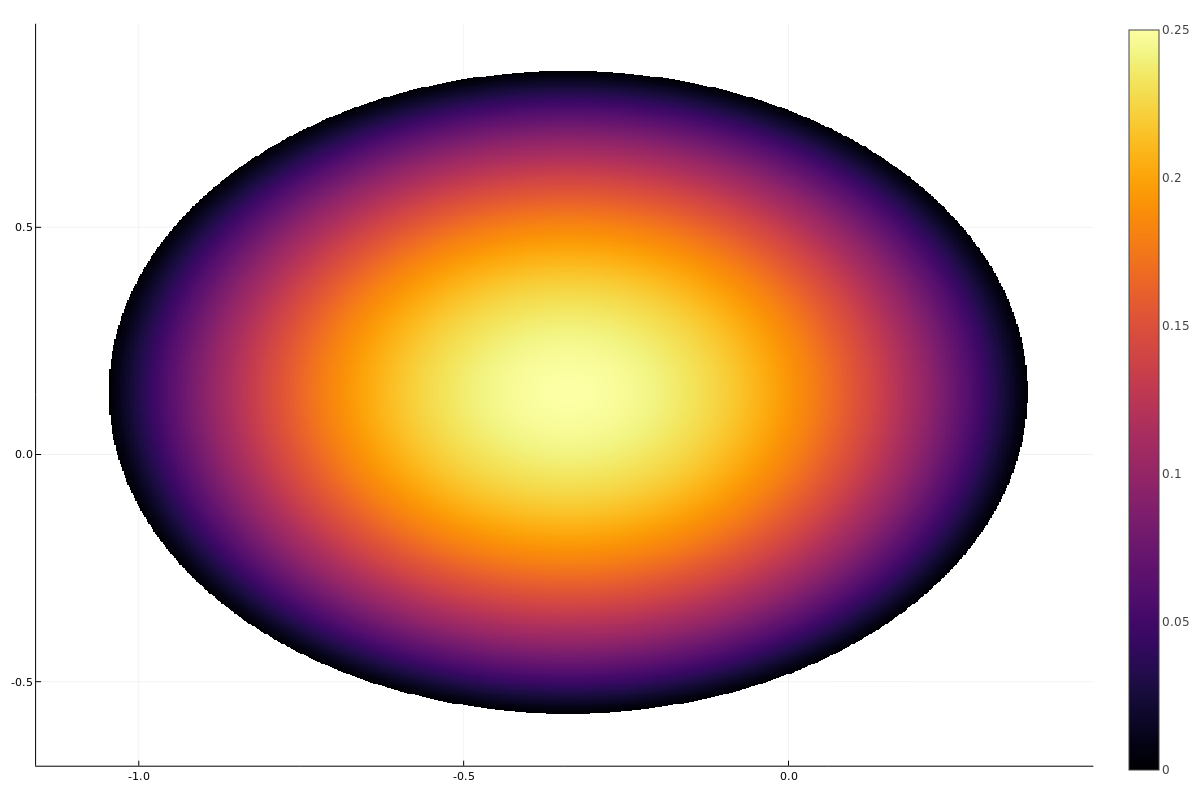
\includegraphics[width=0.99\textwidth]{det2.png}
    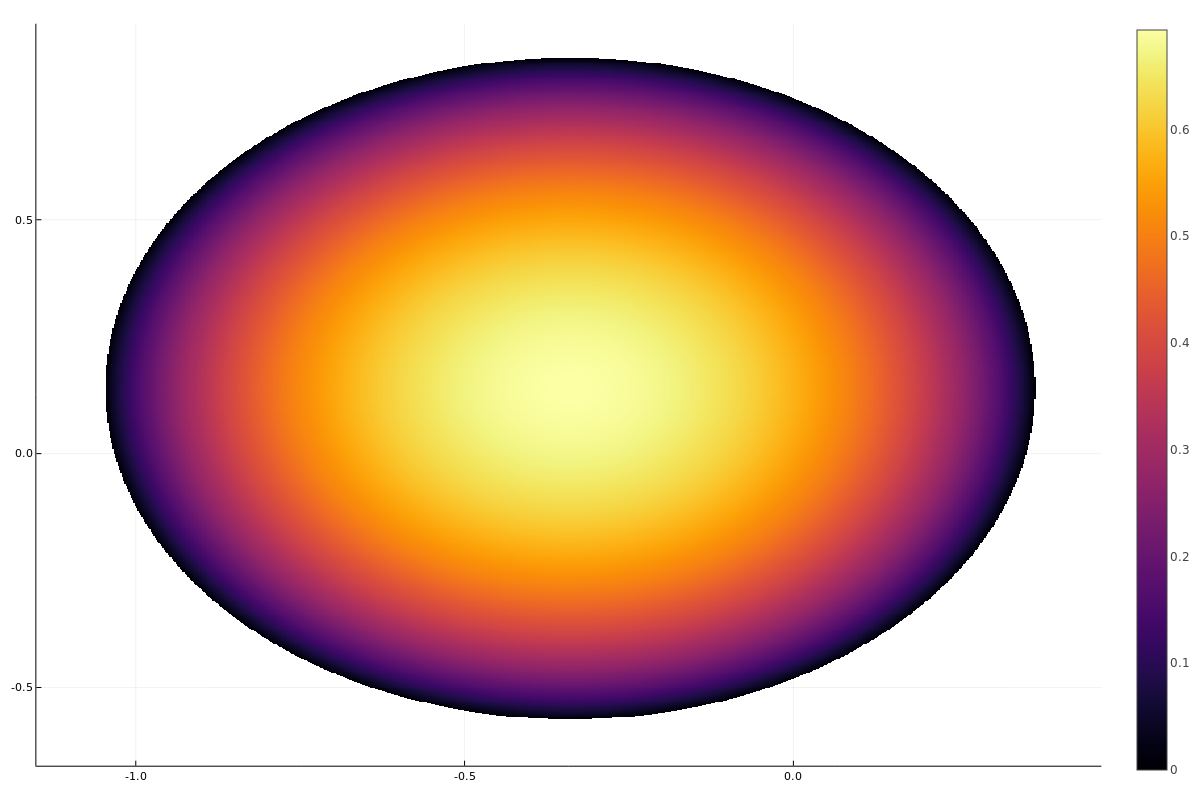
\includegraphics[width=0.99\textwidth]{ent2.png}
    \caption{dimension 2}

  \end{subfigure}
  \begin{subfigure}[t]{0.49\textwidth}
    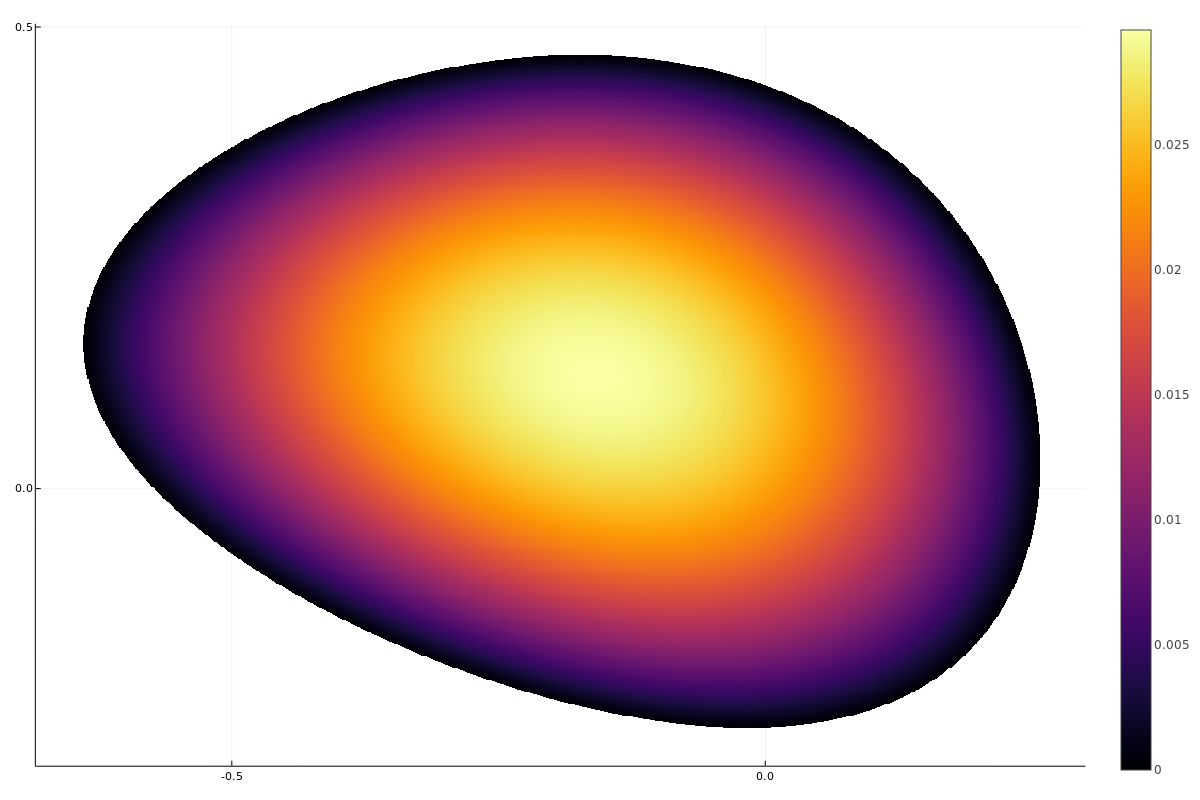
\includegraphics[width=0.99\textwidth]{det3b.png}
    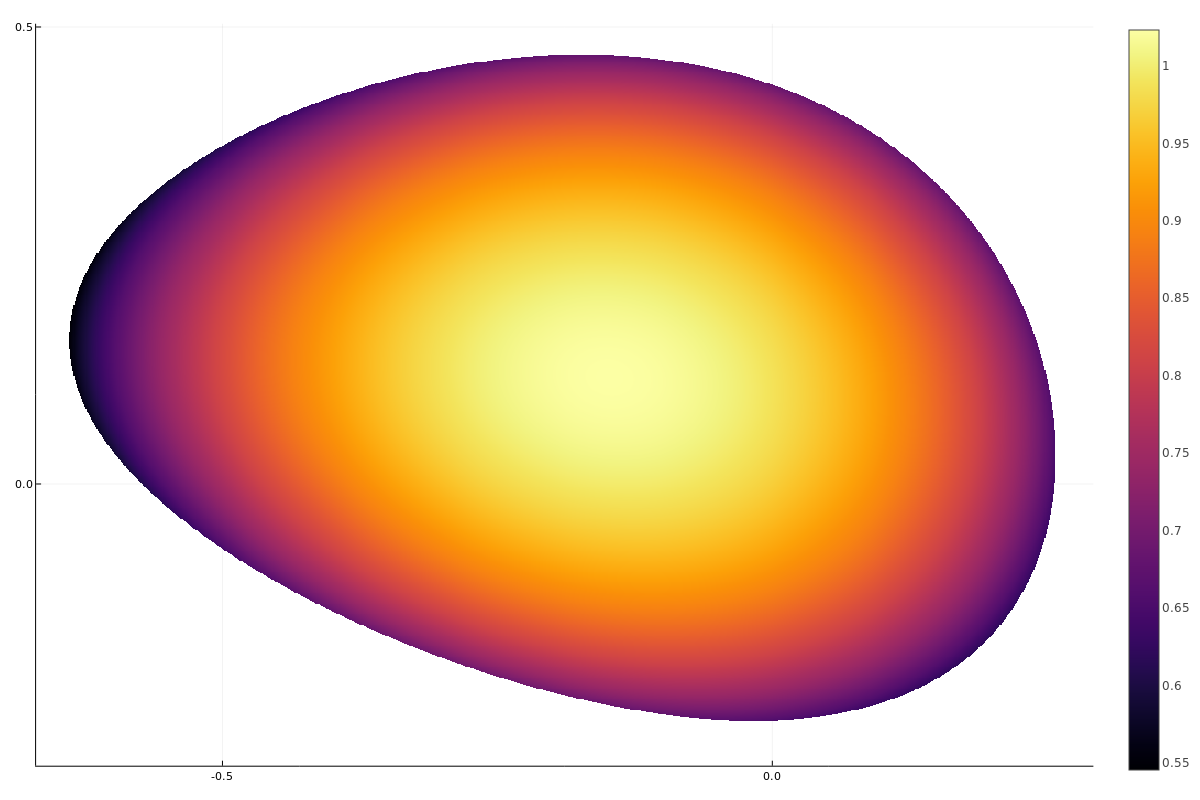
\includegraphics[width=0.99\textwidth]{ent3b.png}
    \caption{dimension 3}
  \end{subfigure}
  \begin{subfigure}[t]{0.49\textwidth}
    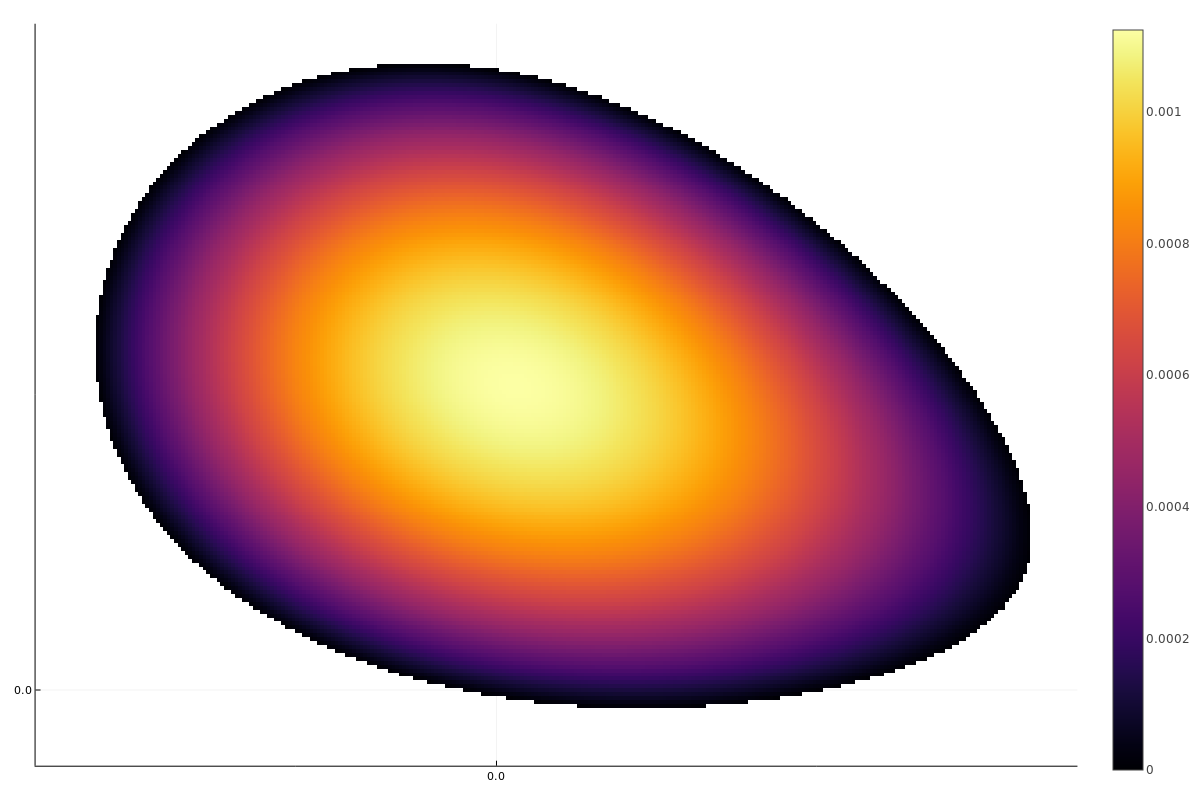
\includegraphics[width=0.99\textwidth]{det4.png}
    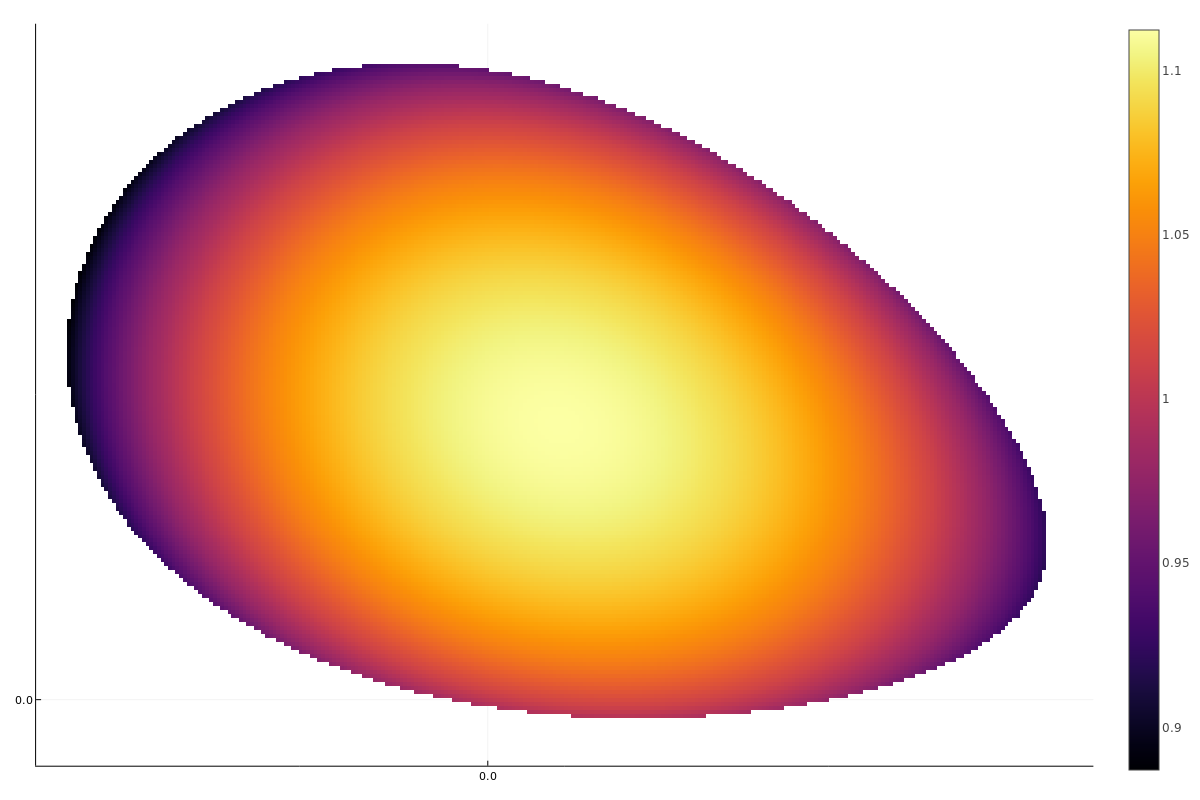
\includegraphics[width=0.99\textwidth]{ent4.png}

    \caption{dimension 4}
  \end{subfigure}
  \begin{subfigure}[t]{0.49\textwidth}
    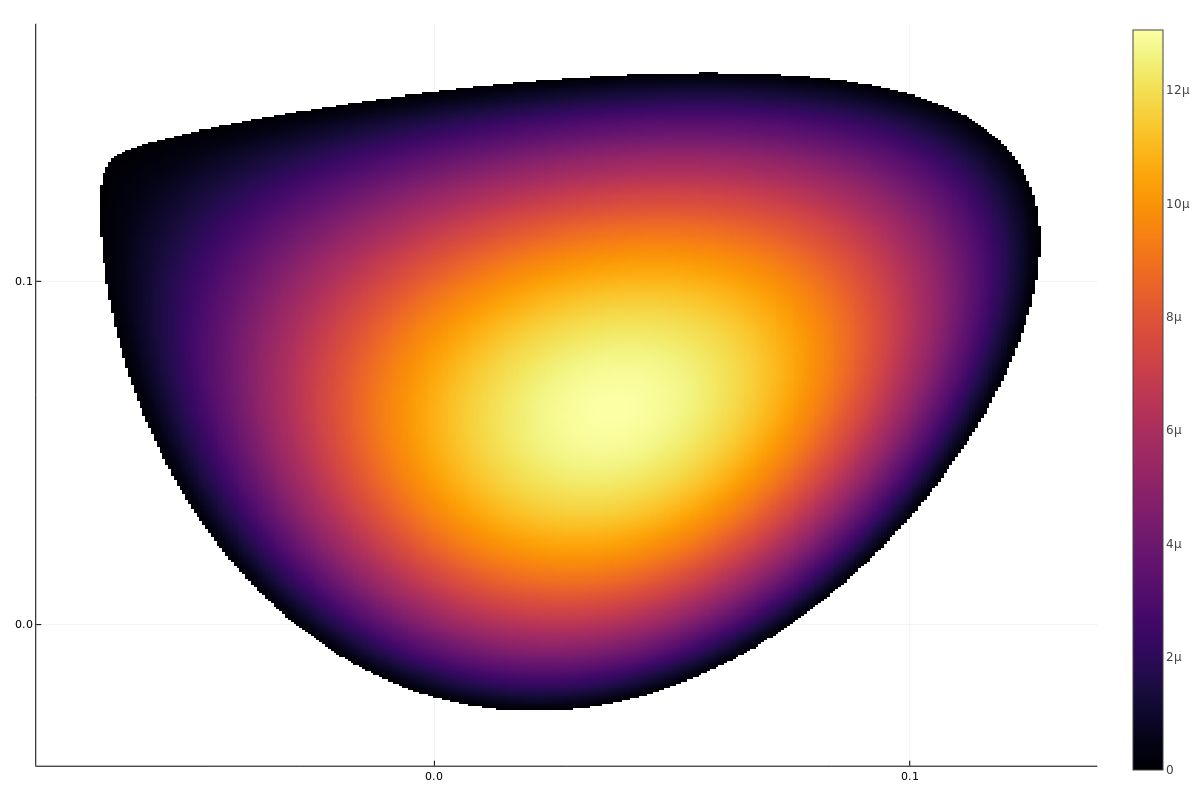
\includegraphics[width=0.99\textwidth]{det5.png}
    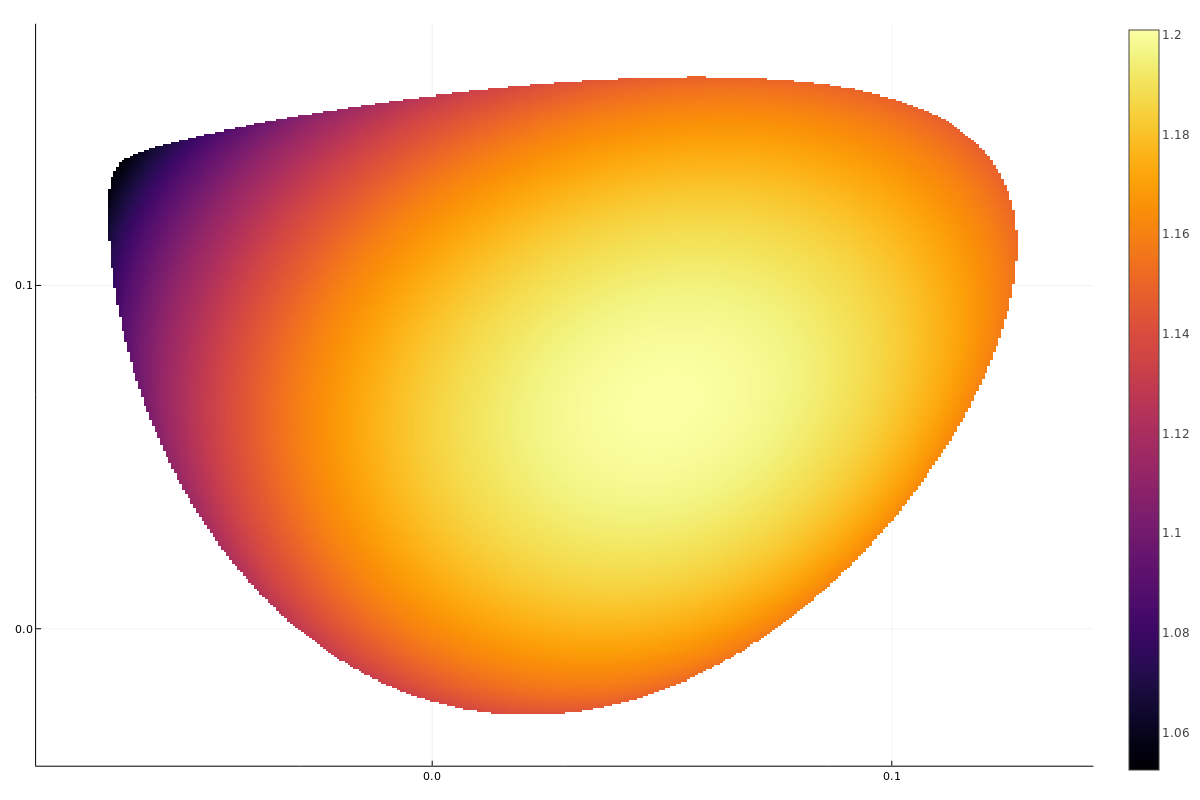
\includegraphics[width=0.99\textwidth]{ent5.png}
    \caption{dimension 5}
  \end{subfigure}

\caption{In order to compare $\log \circ \det$ and $S$, I plotted them on random affine planes
slicing $\mathcal{D}$. I pick a random density matrix $A$ and two random orthonormal null
trace matrices $H_1$ and $H_2$. I then plot $\log \circ \det$ and $S$ in the
plane $A + x H_1 + y H_2$. In each case $\log\circ \det$ is on top and the
entropy is below. The colorless area is outside of $\mathcal{D}$}
\label{fig:heat}
\end{figure}

\subsubsection{In practice}

That part of my work wasn't directly useful for Luis project, because his effect
matrices only span the populations of Fock base and thus the centering simply
consists in putting $0$ in each correlation, which I think achieve perfect centering
whatever the centering function is.

\subsection{Two objective optimisation}

In order to use the centering function, what we want to do is that, after
optimizing $\ell$ and landing on $M = \argmax_{\rho \in \mathcal{D}} \ell(\rho)$, we
can optimize the centering function on $M$ and get the most centered matrix that
maximize $\ell$.

One way of doing it is to do exactly what I just said: Find a $\rho_{int}$ in
$M$ with a first optimization (projected gradient ascent will find one).
Then we could optimize $c$ on $M$.
However I have no idea how to project a vector on $M$: The projection method
described in \cref{ssec:proj} only works on the whole $\mathcal{D}$ because
$\mathcal{D}$ is unitary invariant which is generally not the case of $M$.

An other way of doing that is by using a kind of barrier method with $c$. By optimizing $\ell +
\varepsilon c$ and reducing progressively $\varepsilon$, we'll the right
$\rho\ml = \argmax_{\rho \in M} c$.

\begin{prop}
  If I name $\rho_\varepsilon$ the solution of:
  \[\maximf{\ell + \varepsilon c}{\rho \in \mathcal{D}}\]

  Then, if $c$ is strictly concave, and uniformly continuous we'll have:

  \[ \rho_\varepsilon \xrightarrow[\varepsilon \to 0]{} \rho\ml = \argmax_{\rho \in M} c\]
\end{prop}

\begin{proof}
  Let's define $\ell\ml = \ell(\rho\ml)$.
  $\ell$ is strictly concave on all the dimension on which there is an $E_i$
  i.e all the dimension orthogonal to $M$. That means that if
  $\ell(\rho_\varepsilon) \to \ell\ml$, then $d(\rho_\varepsilon,M) \to 0$.

  Then lets prove that $\ell(\rho_\varepsilon) \to \ell\ml$. We now that
  $\ell\ml > \ell(\rho_\varepsilon)$, but we also know that
  $\ell(\rho_\varepsilon) + \varepsilon c(\rho_\varepsilon) \geq \ell\ml +
  \varepsilon c(\rho\ml)$. Therefore:
  \[\ell\ml - \ell(\rho_\varepsilon) < \varepsilon (g(\rho_\varepsilon) - g(\rho\ml))\]
  But $c$ is strictly concave so it has an upper bound. So when $\varepsilon \to
  0$, we have $\ell\ml - \ell(\rho_\varepsilon) \to 0$ and thus
  $d(\rho_\varepsilon,M)\to 0$.

  Let's name $\rho_{p\varepsilon}$ the projection of $\rho_\varepsilon$ on $M$.
  As $\rho_{p\varepsilon} \in M$, we have $g(\rho_{p\varepsilon}) < c(\rho\ml)$.

  By uniform continuity, $d(g(\rho_{p\varepsilon}),c(\rho_\varepsilon)) \to 0$
  and $g(\rho\ml)$ is between them so $c(\rho_{p\varepsilon}) \to c(\rho\ml)$.
  But as $c$ is strictly concave, this must mean that $\rho_{p\varepsilon} \to
  \rho\ml$.

  On the other hand we had $d(\rho_\varepsilon,M) =
  d(\rho_\varepsilon,\rho_{p\varepsilon}) \to 0$, so in the end we have
  $\rho_\varepsilon \to \rho\ml$.
\end{proof}

This proof works perfectly with the entropy but not with the $\log \circ \det$
as it isn't uniformly continuous. Furthermore, the projected gradient method won't
work directly with the entropy because when projecting on the edge, the gradient of the
entropy will be infinite. I think both of this problems have solutions, for
example when we are on the edge, only output the tangent gradient for the
entropy. However, the internship is finished, so I won't have the time to check
it properly.



Centering functions.


\section{Conclusion}

\TODO Write it

\bibliographystyle{plain}

\bibliography{article}


\newpage\appendix

{\huge Appendix}

\vspace{1cm}

\section{Morse lemma}

\begin{lem}\label{lem:dec}
  Let $f : U \subset \R^n \to \R^m$, be $\class{n}$ with $U$ a neighborhood of 0.
  Suppose that $f(0) = 0$. Then we have $g : U \to \mathcal{L}(\R^n,\R^m)$ of
  class $\class {n-1}$ such
  that:
  \[f(x) = g(x) x\]
  and with $g(0) = \nabla f(0)$
\end{lem}

\begin{proof}
  $g(x) = \int_0^1 \nabla f(tx) \dd t$
\end{proof}

\begin{lem}\label{lem:dec2}
  Let $f : U \subset \R^n \to \R$, be $\class{n}$ with $U$ a neighborhood of 0.
  Suppose that $f(0) = 0$ and $\nabla f(0) = 0$.
  Then we have $h : U \to \mathcal{S}(\R^n)$ of class
  $\class {n-2}$ such
  that $h(0) = \nabla^2 f(0)$ and:
  \[f(x) = \bra x h(x) \ket x\]
\end{lem}

\begin{proof}
  We apply \cref{lem:dec} on $f$ to get $g$, that we see as a gradient $g :U \to
  \R^n$. Then we apply it again on $g$ to get $h_0$, then we take the symmetric part:
  \[h = \frac{h_0 + h_0^t}2\]

  We also have: $h_0(0) = \nabla g(0) = \nabla^2 f(0) = h(0)$
\end{proof}


\begin{lem}[Morse lemma]\label{lem:morse}
  Let $f : U \subset \R^n \to \R$, be $\class{n}$ with $U $ a neighborhood of 0.
  Suppose that $f(0) = 0$, $\nabla f(0) = 0$ and $\nabla^2 f > 0$.
  Then we have a neighborhood $V$ of 0 and $\psi : V \to \R^n$ of class
  $\class{n-2}$, a such that on $V$:
  \[f(x) = \|\psi(x)\|^2\]

  If $n \geq 3$, we can have $\psi$ a diffeomorphism with $\nabla \psi(0) = \sqrt{\nabla^2 f(0)}$
\end{lem}

\begin{proof}
  We take $h$ as in \cref{lem:dec2}. As $h$ is continuous, we can take $V$ such
  that $h > 0$ on $V$ ($h(0) = \nabla^2 f > 0$).

  We can then define $\psi(x) = \sqrt{h(x)} x$. With the square root being the
  $\class{\infty}$ square root on the positive definite matrices.
  If $n \geq 3$, then $h$ is $\class 1$, thus we have: $\nabla \psi(0) =
  \sqrt{h(0)} = \sqrt{\nabla^2 f(0)}$. As $\nabla^2
  f(0) > 0$, we have $\nabla \psi(0)$ invertible, so by local inversion theorem,
  we can reduce the size of $V$ to make $\psi$ a diffeomorphism on $V$.

\end{proof}






\end{document}
